\documentclass[autodetect-engine,dvipdfmx-if-dvi,ja=standard,a4j,jbase=11pt,magstyle=nomag*]{bxjsreport}
% \documentclass[uplatex, dvipdfmx, a4paper, 11ptj, report]{jsbook}
% small japanese font size:     9pt, 10pt, 11pt, 12pt, 14pt, ... (please refer the document of jsclasses)
% word-like japanese font size: 10ptj 10.5ptj, 11ptj, 12ptj (or jbase=xxpt (without 'j') if error is occured)

\usepackage{ifptex,ifxetex,ifluatex}
\ifluatex
    \usepackage{bxcalcux}
    \ltjsetparameter{jacharrange={-2,-3}}
    \usepackage{luatexja-otf}
    \usepackage{bxbase}
\else\ifxetex
    % \usepackage{zxjatype}
    % \usepackage[macros]{zxotf}
    \XeTeXgenerateactualtext=1
    \usepackage{xltxtra}
    \usepackage{bxbase}
\else\ifuptex
    \usepackage{otf}
    \usepackage[prefernoncjk]{pxcjkcat}
    \cjkcategory{sym11,sym18,sym19}{cjk}
    \usepackage[utf8]{inputenc}
    \usepackage{pxbase}
\else\ifstrictptex
    \usepackage{otf}
    \usepackage[utf8]{inputenc}
    \usepackage{pxbase}
\fi\fi\fi\fi

\usepackage[LGR,T2A,T1]{fontenc}

\usepackage{graphicx}
% \usepackage[dvipdfmx]{graphicx}
\usepackage{grffile}

% paper layout setting
\setpagelayout{noheadfoot, left=18.0truemm, right=18.0truemm, top=29.0truemm, bottom=26.0truemm, columnsep=6.5truemm}
% \setpagelayout{noheadfoot, left=15.0truemm, right=5.0truemm, top=12.5truemm, bottom=12.5truemm, columnsep=5.0truemm}

% font setting
\usepackage{amsmath}
\usepackage{amssymb}
\usepackage{mathtools}
\usepackage{bm}
\usepackage{fix-cm}
\usepackage{newtxtext}
\usepackage[slantedGreek]{newtxmath}

% caption setting
\usepackage[font=bf,labelfont=bf,labelsep=quad]{caption}

% to balance the last page of the two-column article
% \usepackage[nospread, keeplastbox, nodebug]{flushend}

% title font style
\renewcommand{\headfont}{\bfseries}

% section setting (using titlesec, uelm package)
\renewcommand{\thesection}{\arabic{section}}
\renewcommand{\thesubsection}{\arabic{section}.\arabic{subsection}}

\usepackage[explicit]{titlesec}
\usepackage[normalem]{ulem}
\titleformat{name=\section}{\normalfont\headfont\normalsize\raggedright}{}{0pt}{\uline{\thesection.\quad#1}}
\titleformat{name=\section,numberless}{\normalfont\headfont\normalsize\raggedright}{}{0pt}{\uline{#1}}
% \titleformat{name=\section}{\normalfont\headfont\normalsize\raggedright}{}{0pt}{\thesection.\quad#1}
\titlespacing{name=\section}{0pt}{.5\Cvs plus .0\Cvs minus .3\Cvs}{.1\Cvs plus .0\Cvs minus .1\Cvs}
\titleformat{name=\subsection}{\normalfont\headfont\normalsize\raggedright}{}{0pt}{\thesubsection.\quad#1}
\titleformat{name=\subsection,numberless}{\normalfont\headfont\normalsize\raggedright}{}{0pt}{#1}
\titlespacing{name=\subsection}{0pt}{.3\Cvs plus .0\Cvs minus .2\Cvs}{.0\Cvs plus .0\Cvs minus .0\Cvs}

% \makeatletter
% \renewcommand{\section}{\@startsection{section}{1}{\z@}{.5\baselineskip}{.1\baselineskip}{\normalfont\normalsize\headfont\raggedright}}
% \renewcommand{\subsection}{\@startsection{subsection}{2}{\z@}{.3\baselineskip}{\z@}{\normalfont\normalsize\headfont\raggedright}}
% \makeatother

\usepackage{secdot}
\sectiondot{section}
\sectiondot{subsection}

% list (itemize, enumerate, description, ...)
\usepackage{enumitem}
\setlist[1]{parsep=.0\baselineskip,topsep=.2\baselineskip,itemsep=.1\baselineskip}
% \makeatletter
% \def\@listi{\leftmargin\leftmargini
%     \parsep \z@
%     \topsep .2\baselineskip
%     \itemsep .1\baselineskip \relax}
% \let\@listI\@listi
% \makeatother

% no page number
\pagestyle{empty}

% footnote
\usepackage[bottom,hang,stable]{footmisc}
\setlength{\footnotemargin}{0pt}

% float setting (figure, table)
\setlength\floatsep{2.0truemm}
\setlength\textfloatsep{2.0truemm}
\setlength\intextsep{1.0truemm}
\setlength\dblfloatsep{2.0truemm}
\setlength\dbltextfloatsep{2.0truemm}
\setlength\abovecaptionskip{0.5truemm}
\setlength\belowcaptionskip{0.5truemm}

% lineskip setting (body text, display-style equation)
\AtBeginDocument{%
    \narrowbaselines    % basic english lineskip (for article)
    % \widebaselines      % basic japanese lineskip
    %
    \setlength\abovedisplayskip{1.5truemm}    % equation setting
    \setlength\belowdisplayskip{1.5truemm}    % equation setting
}

% to suit ms-word template
\renewcommand{\baselinestretch}{0.9}


\makeatletter
%
% maketitle
% additional elements
\newcommand*{\etitle}[1]{\gdef\@etitle{#1}}
\newcommand*{\studentid}[1]{\gdef\@studentid{#1}}
\newcommand*{\laboarea}[1]{\gdef\@laboarea{#1}}
\newcommand*{\laboname}[1]{\gdef\@laboname{#1}}
%
% style definition
\def\@maketitle{%
\newpage%
\centering%
\let\footnote\thanks%
%
% title
{\fontsize{16.00truept}{16.00truept}\selectfont\headfont\@title\par}%
%
% english title
\ifx\@etitle\@undefined\else{\vspace{1truemm}{\fontsize{12truept}{12truept}\selectfont\headfont\@etitle\par}}\fi%
%
% name (option: student id)
\vspace{1truemm}%
\ifx\@studentid\@undefined\else{\fontsize{12truept}{12truept}\selectfont\headfont\@studentid\hspace{\Cwd}}\fi%
{\fontsize{12truept}{12truept}\selectfont\headfont\@author\par}%
%
% research area (\laboarea) and laboratory name (\laboname)
\ifx\@laboarea\@undefined%
    \ifx\@laboname\@undefined%
    \else\vspace{1truemm}{\fontsize{12truept}{12truept}\selectfont\headfont\@laboname\par}%
    \fi%
\else%
    \ifx\@laboname\@undefined\vspace{1truemm}{\fontsize{12truept}{12truept}\selectfont\headfont\@laboarea\par}%
    \else\vspace{1truemm}{\fontsize{12truept}{12truept}\selectfont\headfont\@laboarea\hspace{\Cwd}\@laboname\par}%
    \fi%
\fi%
%
%% old version (2 line) of research area (\laboarea) and laboratory name (\laboname)
%\ifx\@laboarea\@undefined\else{\vspace{1truemm}{\fontsize{10truept}{10truept}\selectfont\@laboarea\par}}\fi%
%\ifx\@laboname\@undefined\else{\vspace{1truemm}{\fontsize{10truept}{10truept}\selectfont\@laboname\par}}\fi%
%
%% date (error)
% \ifvoid\@date\else{\vspace{2truemm}{\fontsize{12truept}{12truept}\selectfont\@date\par}}\fi%
%
% abstract (no check)
\ifvoid\@abstractbox\else{\vspace{2truemm}{\centering{\fontsize{10truept}{10truept}\selectfont\box\@abstractbox\par}}}\fi%
\vspace{2truemm}%
}
%
%
% bibliography
\newcommand{\@bibsection}{\@startsection{section}{1}{\z@}{.5\baselineskip}{0.2\baselineskip}{\normalfont\fontsize{9truept}{11truept}\selectfont\headfont\raggedright}}
\setlength\bibindent{\Cwd}
\renewenvironment{thebibliography}[1]{%
    \global\let\presectionname\relax
    \global\let\postsectionname\relax
    \@bibsection*{\refname}\@mkboth{\refname}{\refname}%
    \list{\@biblabel{\@arabic\c@enumiv}}{%
        \settowidth\labelwidth{\@biblabel{#1}}%
        \leftmargin\labelwidth
        \advance\leftmargin\labelsep
        \setlength\itemsep{0.5truept plus 1.0truept minus 0.5truept}
        \@openbib@code
        \usecounter{enumiv}%
        \let\p@enumiv\@empty
        \renewcommand\theenumiv{\@arabic\c@enumiv}}%
    \fontsize{8truept}{9.5truept}\selectfont
    \sloppy
    \clubpenalty4000
    \@clubpenalty\clubpenalty
    \widowpenalty4000%
    \sfcode`\.\@m}
{\def\@noitemerr{\@latex@warning{Empty `thebibliography' environment}}\endlist}
%
\makeatother


\mainmatter
\setchapterxr[thesis][bibliography]{3}


\begin{document}


\chapter{複数LiDARの位置校正方法とオクルージョン範囲の導出}
	
\section{はじめに}
本章では,LiDARの位置を取得するために使用した手法を説明する.
また,決定したLiDARの位置とそれが認識した人物の位置からオクルージョンが起こっている範囲を導出し,
その範囲をUAVが撮影できるように目標位置を設定する手法を説明する.

\section{複数LiDARの位置決定方法}
まず始めに,複数LiDARの位置の取得方法について述べる.
先行研究では1台のLiDARの位置をUAVに搭載しているGPSセンサと同じもの使用してを取得していた.
しかし,UAVに搭載されているGPSセンサから得られる緯度経度情報は数mから十数mの誤差がある.
複数のLiDARを使用する際,位置の誤差が大きいと,1つの物体を2つの物体と誤認してしまう恐れがある.
そのため,2つのLiDARの正確な相対位置を取得するためにRTK-GPS測位という手法を利用して位置を取得する.

\subsection{RTK-GPS測位}
RTK-GPS(Real-Time Kinematic GPS)測位とは,位置が分かっていて移動しない基地局(Base)と
位置情報を取得しようとしている観測点である移動局(Rover)で同時にGPS観測を行い,
基準局で観測したデータを移動局へリアルタイムに送信し,基準局の位置に基づいて移動局の位置を求める手法である.
さらにネットワークを利用して基地局と移動局のデータ送信を行うことで,
基地局と移動局が長距離で離れていても精度の高い演算ができる.

\begin{figure}[t]
    \centering
    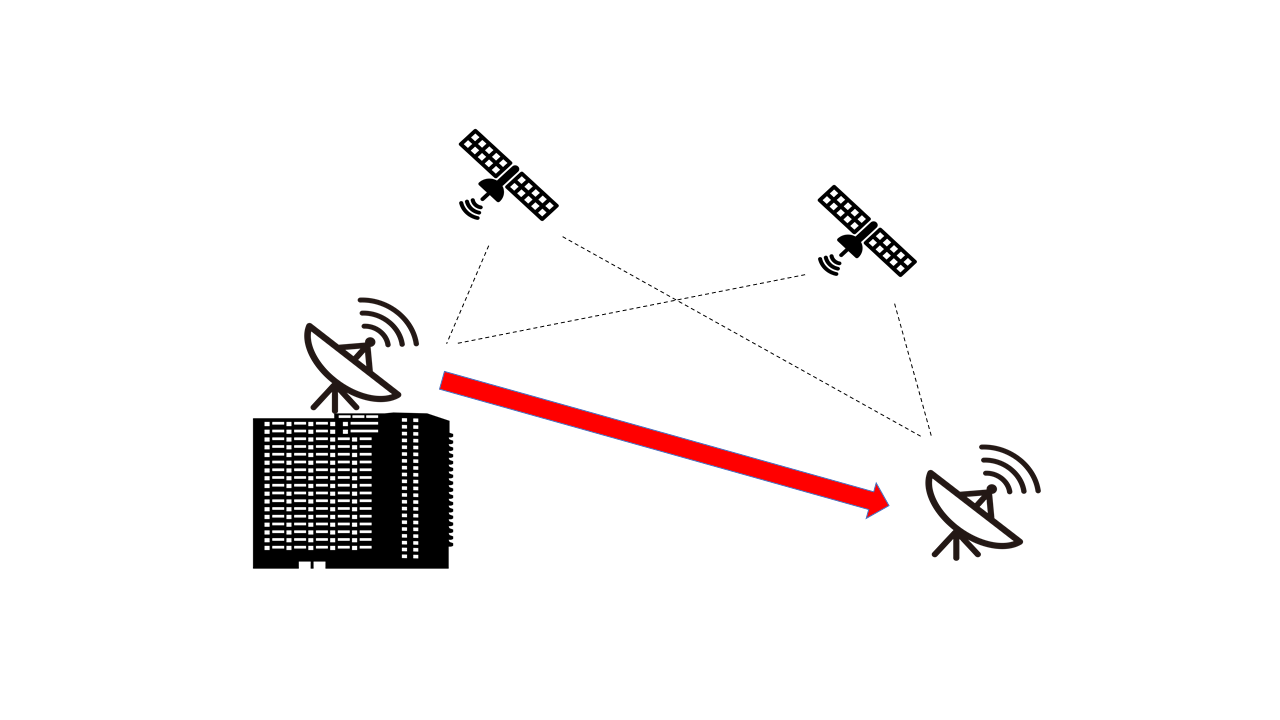
\includegraphics[width=\linewidth, clip]{./figure/chapter3/RTK.png}
    \caption{Image of RTK-GPS Positioning System}
    \label{fig:RTK}
\end{figure}

\subsection{RTK-GPS測位と単独測位の比較}
単独測位では数mから十数mの誤差が発生するのに対して,
RTK-GPS測位では数cmの誤差が発生するといわれている.
ここで,実際に計測したデータを比較して測位の性能の差を述べる.
計測位置は大阪市立大学F棟507号室のベランダであり,\cref{fig:data_of_RTK}は30秒の計測データをグラフ化したものである.
\cref{fig:data_of_RTK}左のグラフは単独測位の結果であり,グラフは1マス50cmである.
同図右のグラフはRTK-GPS測位の結果であり,グラフは1マス1cmである.
グラフはから見て取れるように,単独測位は50cmから1mの誤差があり,
RTK-GPS測位の誤差は1cmから2cm以内に収まっている.

\begin{figure}[t]
    \centering
    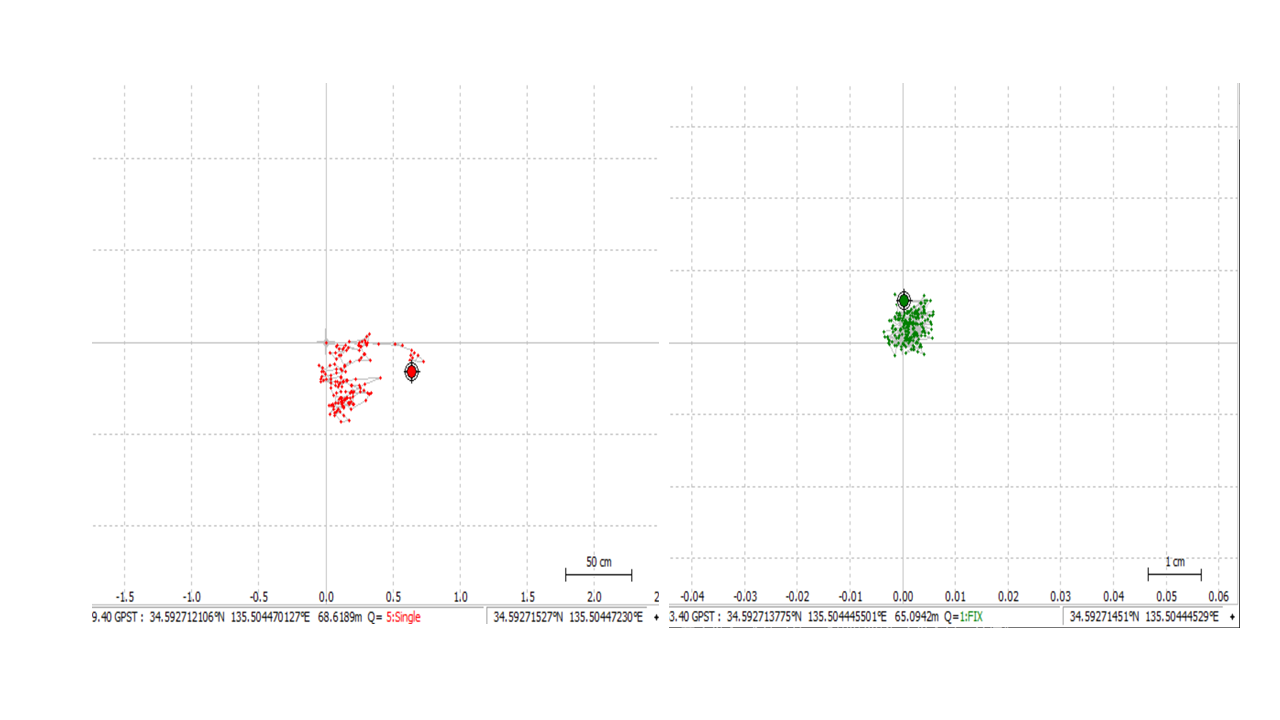
\includegraphics[width=\linewidth, clip]{./figure/chapter3/Data_of_GPS_positioning.png}
    \caption{Single GPS Positioning (right) and RTK-GPS Positioning (left)}
    \label{fig:data_of_RTK}
\end{figure}

\section{GPS座標からmap座標への変換}
本研究では,東を{\it x}座標正方向,北を{\it y}座標正方向とするmap座標系を用いる.
また座標原点はLiDAR1の座標をもとに算出する.
ここでは,GPSセンサから得たLiDAR1の緯度経度と座標から原点の緯度経度の値の算出方法,
原点の緯度経度の値とLiDAR2の緯度経度の値からLiDAR2のmap座標の算出方法を述べる.

LiDAR1のGPS座標を$lon_{lidar1}, lat_{lidar1}$,map座標を$x_{lidar1}, y_{lidar1}$とすると
求めるmap座標原点の緯度経度の値$lon_{origin}, lat_{origin}$は以下の\cref{eq:calc_gps}で算出される.
なお式中の$R$は地球の赤道半径である.

\begin{equation}
    \begin{aligned}
        lat_{origin} &= \frac{y_{lidar1}}{R} \times \frac{180}{\pi} + lat_{lidar1}\\
        lon_{origin} &= \frac{x_{lidar1}}{R} \times \frac{180}{\pi} \times \frac{1}{cos( lat_{origin} \frac{180}{\pi})} + lon_{origin}
    \end{aligned}
    \label{eq:calc_gps}
\end{equation}

\cref{eq:calc_gps}より得られたmap座標原点の緯度経度の値を用いて,
LiDAR2のmap座標$x_{lidar2}, y_{lidar2}$を\cref{eq:calc_from_gps}求めることができる.
LiDAR2のGPS座標を$lon_{lidar2}, lat_{lidar2}$とする.

\begin{equation}
    \begin{aligned}
        x_{lidar2} &=  R ( lon_{lidar2} - lon_{lidar2} ) \frac{\pi}{180} cos(( lat_{lidar2} - lat_{origin} )\frac{\pi}{180}) \\
        y_{lidar2} &=  R ( lat_{llidar2} - lat_{origin} ) \frac{\pi}{180}
    \end{aligned}
    \label{eq:calc_from_gps}
\end{equation}

\section{オクルージョンが発生した場合のUAVの撮影位置の決定}
前節まででは,LiDARの位置を取得するための手法を述べた.
人物行動範囲内に複数人の人物が存在する場合,オクルージョンが発生し.
地上設置LiDARでは人物行動範囲内の全ての人物をとらえきれない場合が存在する.
この節では,オクルージョンが発生した場合のLiDARの撮影できない領域と,
その領域を考慮したUAVの目標位置の導出方法について述べる.

 
       .

\subsection{数値計算安定化のための各種パラメータ設定方法}
問題で用いる係数行列およびベクトルを次のように設定することで,反復計算の安定性および収束性能を向上させる.
\begin{itemize}
    \item   $K_p$,$K_u$,$K_{u_z}$の各成分を,係るベクトルの各要素をそれぞれ最大値で正規化するように設定する
\end{itemize}
\begin{equation} \label{eq:Kp_setting}
    \begin{aligned}
        K_p & = \mathrm{diag} \, \{ k_x , k_y , k_{\theta} , k_l , k_{\theta_{fl}} , k_{\theta_{fr}} \} \\
        & k_x = k_y = ( \max \{ | x_{\goal} - x^0 | , | y_{\goal} - y^0 | \} )^{-2} \\
        & k_{\theta} = ( 2 \pi )^{-2} \\
        & k_l = ( Y_{\mathrm{max}} - Y_{\mathrm{min}} )^{-2} \\
        & k_{\theta_{fl}} = k_{\theta_{fr}} = ( 2 \pi )^{-2}
    \end{aligned}
\end{equation}
\begin{equation} \label{eq:Ku_setting}
    \begin{aligned}
        K_u & = \mathrm{diag} \, \{ \dots , k_{u_A} , k_{u_B} , k_{u_{l1}} , k_{u_{l2}} , k_{u_{fl}} , k_{u_{fr}} , \dots \} \\
        & k_{u_A} = k_{u_B} = ( 2 \tan^{-1} ( X_{\mathrm{max}} / Y_{\mathrm{min}} ) + {\theta_2}_{\mathrm{max}} )^{-2} \\
        & k_{u_{l1}} = k_{u_{l2}} = ( Y_{\mathrm{max}} - Y_{\mathrm{min}} )^{-2} \\
        & k_{u_{fl}} = k_{u_{fr}} = ( {\theta_2}_{\mathrm{max}} - {\theta_2}_{\mathrm{min}} )^{-2}
    \end{aligned}
\end{equation}
\begin{equation} \label{eq:Kuz_setting}
    \begin{aligned}
        K_u & = \mathrm{diag} \, \{ \dots , k_{u_{zl}} , k_{u_{zr}} , \dots \} \\
        & k_{u_{zl}} = k_{u_{zr}} = z_{\mathrm{max}}^{-2}
    \end{aligned}
\end{equation}
\begin{itemize}
    \item   $K_u$,$K_{u_z}$は,前項の設定に加えてSugiharaの手法~\cite{sugihara_2011tro}を適用し,
            評価関数\cref{eq:evaluation_function}の値を用いて重み付けする
            ($I$は単位行列,$\Delta k_u$はスカラー定数)
\end{itemize}
\begin{equation}
    \label{eq:LM_Kuset_sugihara}
    \begin{gathered}
        K_u \gets V_{\now} \, K_u + \Delta k_u \, I = \frac{1}{2} {\left\| \bm{\varepsilon}_{\now} \right\|}^2_{K_p} \, K_u + \Delta k_u \, I \\
        K_{u_z} \gets V_{\now} \, K_{u_z} + \Delta k_{u_z} \, I = \frac{1}{2} {\left\| \bm{\varepsilon}_{\now} \right\|}^2_{K_p} \, K_{u_z} + \Delta k_{u_z} \, I
    \end{gathered}
\end{equation}
\begin{itemize}
    \item   一つ一つの制約条件$\omega_i(\bm{q}^0 ,\, \bm{U}_k) \geq 0$を$\| \nabla \omega_i \|$で正規化することにより,
            GI法内部での反復計算を安定化させ,また緩和問題での各制約条件の比重を揃える\cite{sugimoto_1985}
    \item   緩和問題を解く際,評価関数全体を$\| \bm{\phi} \|$で正規化し,
            元の評価関数部分の値とスラック変数の値の比重を揃える($\rho = 1$とできる)
\end{itemize}
そして,得られた解を用いてArmijoの基準に基づく直線探索を行い,入力列を更新する.



\subsection{直線探索}
直線探索では,次式を満たすステップ幅$\alpha$を求める.
\begin{align}
    \label{eq:armijo}
    \begin{aligned}
        H \left( \bm{q}^0 , \bm{U}_k + \alpha \bm{\Delta U}_k \right) & \leq H \left( \bm{q}^0 , \bm{U}_k \right) + \beta \alpha {\nabla V \left( \bm{q}^0 , \bm{U}_k  \right)}^T \bm{\Delta U}_k \\
                                                                      &   =  H \left( \bm{q}^0 , \bm{U}_k \right) + \beta \alpha \bm{\phi}^T \bm{\Delta U}_k
    \end{aligned}
\end{align}
$\beta$は,$0 < \beta < 1$を満たす定数である.
今回,$\alpha$は\cref{fig:algorithm_linesearch}に示す単純な探索により求める.
なお,$\gamma$は$0 < \gamma < 1$を満たす減衰係数である.


\section{終了判定}
更新後,終了判定を行う.
次の項目を\emph{すべて}満たすことを終了条件とする.
\begin{itemize}
    \item   $\bm{\varepsilon}$が収束(各要素が許容誤差$\bm{\varepsilon}_{\goal}$の各要素よりも小さい)
    \item   $\bm{\Delta U}_k$が収束(各要素が許容誤差$\bm{\varepsilon}_{\mathrm{input}}$の各要素よりも小さい)
    \item   $\omega_i(\bm{q}^0 ,\, \bm{U}_k) \geq 0 \ (i = 0 , \dots ,\, 20k - 1)$をすべて満たす
\end{itemize}
これらの条件を全て満たしていれば,その時点での$\bm{U}_k$を解とし,計画を終了する.
満たしていない場合は次節の処理へ移る.

\section{目標到達可否判定}
初期ステップ数$k_\mathrm{init}$は直線距離から算出するため,現在の$k$では歩数不足の場合がある.
そこで,反復毎に目標状態へ収束する見込みがあるかどうかを判定し,見込みがない場合に$k$を増やす処理を行う.
ここでは,次の項目の\emph{いずれか}を満たせば到達不可と判定することとする.
\begin{itemize}
    \item   ``$\bm{\Delta U}_k$収束時に$\bm{\varepsilon}$が未収束'' という状況が$n_{\reachable1}$回繰り返される
    \item   現在の$k$における反復回数$\mathrm{loop}$が$n_{\reachable2}$に達した段階で,
   $\bm{\varepsilon}$が大きい値をとる(各要素が到達見込みの閾値$\bm{\varepsilon}_{\reachable}$の各要素よりも大きい)
\end{itemize}
到達不可と判定された場合には$k \gets k + 1$とし,
また$\bm{U}_k$はその内容を引き継ぎ$\bm{U}_k \gets ( \bm{U}_k^T ,\, \bm{0}^T )^T$として再度反復を開始する.
そうでなければ,``Solve QPP''へ戻り反復を継続する.


\section{地形情報の構築}
\label{sec:z_field_constructure}
前述の計画アルゴリズムを開始する前に,
地形適応制約で用いる地形情報$z_\mathrm{field}(x ,\, y)$を構築する必要がある.
深度カメラや測域センサから得られる点群データを用いて地形情報を構築することを想定し,
次の手順で点群データからの構築を行った.
\begin{enumerate}
    \item   $xy$平面を等間隔に幅$D_\mathrm{grid}$四方の正方形グリッドで分割する.
    \item   各グリッドの領域に含まれるサンプルデータ群の$z$軸成分の平均値を,グリッド中央における高さとする.
    \item   $x ,\, y$方向それぞれについて,グリッド中心の点列をサンプルとする3次スプライン補間関数を計算.
    \item   $z_{\field} ( x ,\, y ) ,\, \partial z_{\field} / \partial x ,\, \partial z_{\field} / \partial y$は,
    与えられた点$( x ,\, y )$に対して直近の$x$軸方向$2$本,$y$軸方向$2$本の補間関数上の値の距離重み付け平均で算出する.
\end{enumerate}
なお,シミュレーションにおいて関数からサンプリングを行って点群データを得る場合,$D_\mathrm{sample}$間隔でサンプリングを行う.


\section{本章のまとめ}
本章では,二次計画法を用いた反復法による脚配置計画問題の求解アルゴリズムの要素として,
必要歩数の推定から毎回の二次計画問題の求解と緩和問題の設定,収束判定,
収束見込み判定とステップ数追加について説明した.
また,地形の違いなどにより問題ごとに大きく変化してしまうことを
可能な限り回避するため,反復法における数値計算の性能を安定させる
重み行列の設定方法などについても述べた.

次章以降は,提案する脚配置計画手法の有用性および性能を検証するための
計画シミュレーションおよび実機実験について述べていく.


\end{document}
